%& -shell-escape

% Les packages utilise's ci-dessous le sont a` titre indicatif ;
% vous pouvez les changer a` votre convenance.

% Le type de document: article, rapport...
\documentclass[a4paper]{report}

% Mettre les diffe'rents packages et fonctions que l'on utilise
%\usepackage[english]{babel}
%\usepackage[french]{babel}
%\usepackage{amsmath}
%\usepackage{amssymb}
%\usepackage{graphics,color}

% Commenter l'une de ces deux lignes
%\RequirePackage[applemac]{inputenc}
%\RequirePackage[latin1]{inputenc}

\usepackage[utf8]{inputenc}
\usepackage[english]{babel}
%\usepackage[francais]{babel}
\usepackage[T1]{fontenc}
%\usepackage{amsmath}
\usepackage{amsfonts}
\usepackage{amssymb}
\usepackage{placeins}
\usepackage{listings}
\usepackage{color}
\usepackage{textcomp}

%----- Package français
%\usepackage[utf8]{inputenc} %reconnaissance des accents
%\usepackage[francais]{babel} %document en français
%\usepackage[T1]{fontenc} %codage des fonts TeX ?



%----- math
\usepackage{amsmath}
\usepackage{dsfont}
\usepackage{calrsfs}

%----- images
\usepackage{graphicx}

%----- dot graphs
\usepackage{pgf}
\usepackage{tikz}
\usetikzlibrary{shapes,arrows}
%\usepackage[debug]{dot2texi}



%\title{Automatic test case generation for java}
%\author{Thomas BRIEN}
%\date{27 Mai 2013}

\begin{document}
%\maketitle

% Titre du rapport
\def\TitreRapport{
    Automatic test generation\\
    for OO programs
}

% Pre'nom et nom dde l'auteur
\def\NomsAuteurs{
    Thomas BRIEN
}

% Date du rapport (dans la me^me langue que le titre)
\def\DateRapport{
    27 Mai 2013
}

% Nom des encadrants
\def\Encadrants{
    \textbf{Encadrant(s)} \\
    Arnaud MAKALA
}
% Nom du laboratoire
\def\Labo{
    Sopra Banking Software - R\&D
}

% mots clef
\def\keyWords{
    automatic test generation, ioLTS/ioPDS, FSM/EFSM, SMT solvers.
}



% Re'sume' en franc,ais avec mots-cle's
\def\ResumeFrancais{
    Nous nous intéressons ici à l'automatisation des de la génération des cas de tests pour les programmes orientés objets. Le travaille effectué concerne les programmes java, les principes exposés s'applique à tout programme orienté objet.\\
    Il existe déjà des outils de génération de tests. Le travail qui suit est un état de l'art des techniques existantes et une proposition de théorie/prototype basé sur les solveurs SMT.
    \\[2mm]
    {\bf Mots-cl\'es : } \keyWords
}

\def\Resume{
    Summary...
    \\[2mm]
    {\bf Key-words : } \keyWords
}


\thispagestyle{empty}
\begin{center}
\baselineskip=1.3\normalbaselineskip
{\bf\Large \TitreRapport}\\[8mm]
{\bf\large \NomsAuteurs}\\[1mm]
{\Labo}\\[4mm]
\DateRapport\\[4mm]
\Encadrants\\[10mm]

\newpage
{\bf R\'esum\'e}
\end{center}


\ResumeFrancais\\[4mm]
\newline
\begin{center}
{\bf Summary}
\end{center}
\Resume\\[4mm]

\newpage


\tableofcontents

\renewcommand{\thesection}{\arabic{section}}

\newtheorem{theorem}{Theorem}
\newtheorem{lemma}{Lemme}

\renewcommand{\thetheorem}{\empty{}}
\renewcommand{\thelemma}{\empty{}} 

\newenvironment{proof}[1][Proof]{\begin{trivlist}
\item[\hskip \labelsep {\bfseries #1}]}{\end{trivlist}}
\newenvironment{definition}[1][Definition]{\begin{trivlist}
\item[\hskip \labelsep {\bfseries #1}]}{\end{trivlist}}
\newenvironment{example}[1][Example]{\begin{trivlist}
\item[\hskip \labelsep {\bfseries #1}]}{\end{trivlist}}
\newenvironment{remark}[1][Rq:]{\begin{trivlist}
\item[\hskip \labelsep {\bfseries #1}]}{\end{trivlist}}
\newenvironment{rappel}[1][rappel:]{\begin{trivlist}
\item[\hskip \labelsep {\bfseries #1}]}{\end{trivlist}}


\chapter*{Introduction}
\addcontentsline{toc}{chapter}{Introduction}




%\chapter*{Plate-forme cible}
%\addcontentsline{toc}{chapter}{Plate-forme cible}




\chapter*{State of the art}
\addcontentsline{toc}{chapter}{State of the art}


\section*{Tests with JUnit}
\addcontentsline{toc}{section}{Tests with JUnit}

\subsection*{Unit tests}
\addcontentsline{toc}{subsection}{Unit tests}
Les tests unitaires ont pour but de prouver la validité d'un objet. Par exemple, on souhaite parcourir la totalité du code en lançant le programme avec des valeurs clef choisies par le programmeur chargé des tests.

\subsection*{Integration tests}
\addcontentsline{toc}{subsection}{Integration tests}
Les tests d'intégration visent à valider la bonne interaction entre plusieurs composants du système.

\subsection*{System tests}
\addcontentsline{toc}{subsection}{System tests}
Comme on peut s'en douter, les tests système permettent de contrôler le système dans son ensemble.

%\section*{Testing by contract}
%\addcontentsline{toc}{section}{Testing by contract}
%L'introduction de contrats dans le code permet de définir les conditions de début, de fin, et les constantes d'exécution.

\section*{Mutation testing}
\addcontentsline{toc}{section}{Mutation testing}
Mutation testing is a method that mesures the "quality" of a test suite.\\
As detailed in $[2.1]$, the methode consists in introducing small modification in the systeme (ex: switch a "+" into a "-") and run the test suite on the modified system, also called the mutant. If the test suite raises an failure, the mutant is "killed".\\
Of course, a test suite should test every possible action of the system and thus, should kill 100\% of mutants.

\section*{Test automation}
\addcontentsline{toc}{section}{Test automation}
- IOCO théorie\\
- ioLTS\\
- FSM/EFSM (Extended Finit State Machin)\\
- MBT (Model-Based Testing)\\
- SMT solvers (yices)\\




\chapter*{Idées et mise en œuvre}
\addcontentsline{toc}{chapter}{Idées et mise en œuvre}
- random testing\\
- dynamic path construction leaded by coverage (récursive)\\
- logic modelisation (FOL) and SMT solver\\

On raisonne sur le code source, et plus particulièrement sur des blocs de code. A partir de ce point, nous appellerons fonction élémentaire une partie de code dont la séquence d'exécution ne dépend d'aucune variable. Plus précisément, un code java qui ne contient pas d'accolades.\\
\newline
Par exemple, le code java suivant contient deux actions elementaires: val=arg1 et val+=arg2\\

\begin{lstlisting}
public int exemple(int arg1, int arg2){
		int val = 0;
		if(this.a<arg1){
			val = arg1;
		}
		if(val<arg2){
			val += arg2;
		}
		return val;
	}
\end{lstlisting}
A cette fonction, on associera le graph suivant:\\


\begin{figure}[h!]
   \caption{\label{étiquette} titre}
   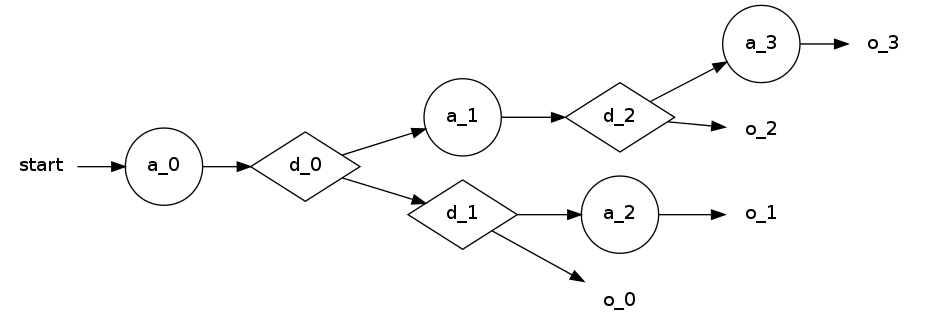
\includegraphics[scale=0.3]{../graphviz/doubleStackGraph.png}
\end{figure}
%\newline



En suivant notre modélisation, on obtient deux actions élémentaires:


\chapter*{Réalisations}
\addcontentsline{toc}{chapter}{Réalisations}


\chapter*{References}
\addcontentsline{toc}{chapter}{References}
\section*{BDD}
\addcontentsline{toc}{section}{BDD}
$[1.1]$ \textit{Testing by Contract
- Combining Unit Testing and Design by Contract}\\
Per Madsen (madsen@cs.auc.dk)
Institute of Computer Science, Aalborg University
Fredrik Bajers Vej 7, DK-9220 Aalborg, Denmark\\
\newline



\section*{Mutation testing}
\addcontentsline{toc}{section}{Mutation testing}
$[2.1]$ \textit{Composants objets fiables :
une approche pragmatique}\\
Daniel Deveaux* - Régis Fleurquin* - Patrice Frison*
Jean-Marc Jézéquel** - Yves Le Traon**\\
* Laboratoire VALORIA (Aglae)
UBS - IUP de Tohannic - Rue Mainguy
56000 VANNES\\
** IRISA-CNRS (Pampa)
Université Rennes 1 - Campus de Beaulieu
35042 RENNES\\
\newline

\section*{Automatisation}
\addcontentsline{toc}{section}{Automatisation}

$[3.1]$ Bertrand Meyer, Ilinca Ciupa, Andreas Leitner and Lisa (Ling) Liu, \textit{Automatic Testing of Object-Oriented Software}, in SOFSEM 2007\\
\newline
$[3.2]$ Hans-Gerhard Gross and Arjan Seesing, 
\textit{A Genetic Programming Approach to Automated Test Generation for Object Oriented Software}, Report TUD-SERG-2006-017\\
\newline
$[3.3]$\textit{Higher-Order Test Generation} - 
Patrice Godefroid - 
Microsoft Research\\
\newline


\end{document}